%%%%%%%%%%%%%%%%%%%%%%%%%%%%%%%%%%%%%%%%%%%%%%%%%%%%%%%%%%%%%%%%%%%%%%%%%%%%%
%	e-Yantra, IIT-Bombay

%	Document Author: Abhishek rathore, Gopineedi Harsha Vardhan
%	Date: 8-June,2016 

%%%%%%%%%%%%%%%%%%%%%%%%%%%%%%%%%%%%%%%%%%%%%%%%%%%%%%%%%%%%%%%%%%%%%%%%%%%%%

\documentclass[11pt,a4paper]{article}

\usepackage{graphicx}
\usepackage{caption}
\usepackage{subcaption}
\usepackage{url}
\title{How to make your own gimbal?}
\author{e-Yantra Team}
\date{\today}

\begin{document}
	\maketitle
	\newpage
	\tableofcontents
	\newpage
	\section{How to make your own gimbal?}
	\textbf{Objective} of this tutorial is to demonstrate how one can make his own gimbal. We will start from "What is Gimbal ?" and go through full gimbal making process and show a working Gimbal at the end.
	\section{Prerequisites}
	\begin{itemize}
		\item 3D Design for 3D Printing
		\item Basic idea about gimbal.
	\end{itemize}
	\section{Hardware Requirement}
	\begin{itemize}
		\item Two Vibration and Shock Absorbing Mounts
		\item Gimbal Motor Frame 1
		\item Gimbal Motor Frame 2
		\item Gimbal Motor Frame 3
		\item Camera Fixing Mount
		\item Three Brushless Gimbal Motors
		\item 3 Axis Brushless Gimbal Controller
		\item One MPU6050  Sensor
		\item Four Damping Shock Absorber Balls
		\item Some Hex Button Head Bolts
		\item Compatible Camera
	\end{itemize}
	\section{Software Requirement}
	\begin{itemize}
		\item 3D design software for 3D printing
	\end{itemize}
	\section{Theory and Description}
		
		\subsection{What is Gimbal?}
		\par A gimbal is a pivoted support that allows the rotation of an object about a single axis. A set of three gimbals, one mounted on the other with orthogonal pivot axes, may be used to allow an object mounted on the innermost gimbal to remain independent of the rotation of its support.For example, on a ship, the gyroscopes, shipboard compasses, stoves, and even drink holders typically use gimbals to keep them upright with respect to the horizon despite the ship's pitching and rolling.
		\par A gimbal is a platform that can pivot. It means that instead of being fixed to an unmoving base, an object on a gimbal can rotate along at least one axis. In the world of aeronautics, these axes are roll, pitch and yaw.
		
		\subsection{Roll, Pitch, Yaw Axis}
		It's easiest to understand roll, pitch and yaw by visualizing an object like an airplane. Think of an imaginary line that runs through the front of the plane and out the back. A rotation along this line would result in a roll -- the plane would start doing barrel rolls.
		\par Now imagine another line running through both wings of the plane. A rotation along this line is a change in pitch. The plane either climbs or dives, depending on the direction of the pitch. A full circle would be a loop-the-loop.
		\par Finally, imagine a vertical line that comes out of the top and bottom of the plane. This is the yaw axis. Rotating along this line results in a change in direction for the plane -- either right or left.
		\newline
		\newline
		\begin{center}
			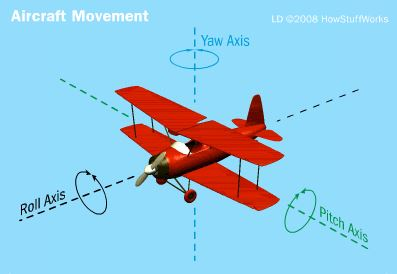
\includegraphics{Aircraft_Movement.JPG}
		\end{center}
		\begin{center}
			\textbf{Figure : Showing Roll, Pitch, Yaw axis in Aircraft}
		\end{center}
		
		\subsection{Gimbal for quadcopter}
		As Drone cannot be perfectly stable either due to poor flying or adverse weather conditions. So here we need gimbal. a gimbal allows you to keep your video recording device stable and fixed. It will aim at the same direction, regardless of whether the craft holding it is pitching forward, left, right, etc.
		\par So a gimbal is used to improve overall image quality, to reduce shakiness in video recordings, and to eliminate the dreaded “jello effect” common on so many videos. Jello-effect (also known as the wobble) appears when the camera is vibrating, in situations such as hand-held shots at telephoto settings, or when shooting from a moving vehicle. The rolling shutter causes the image to wobble unnaturally.
		\newline
		\newline
		\begin{center}
			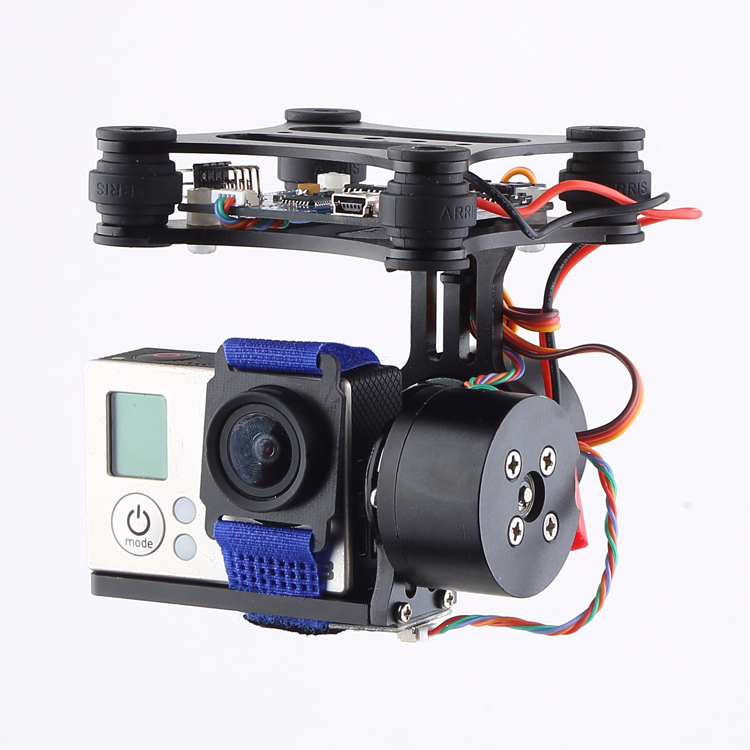
\includegraphics[scale=0.4]{3_Axis_Gimbal_Example.jpg}
		\end{center}
		\begin{center}
			\textbf{Figure : Showing 3 axis gimbal with camera}
		\end{center}
		
		\newpage
		\subsection{Balancing the Gimbal}
		Its important to first balance your gimbal with your camera before you try to tune it as some parameters will change if you are using a different camera.
		\par Its best to first choose what camera/lens you are going to use and try not change it as you will probably need to go through the whole balancing process again if the Centre of Gravity (COG) changes significantly (such as with zoom lens) In general a 14mm to 35mm lens is what you want to use with a gimbal as it gives a nice wide angle. Its also a good idea to put things like camera battery, memory card etc into to the camera before balancing.
		\par Another tip is to attach a quick release mount as its makes life much easier when you need to remove the camera, or put it back on.
		\newline
		\newline
		\textbf{Balance the Pitch axis:}
		\newline
		The first step is to balance the pitch axis. You will need to adjust the height of the camera and also the position (forward/backwards). When its perfectly balanced then when you move the camera to point down slightly, then it will stay there (with no power to motors/gimbal controller).
		\newline
		\begin{center}
			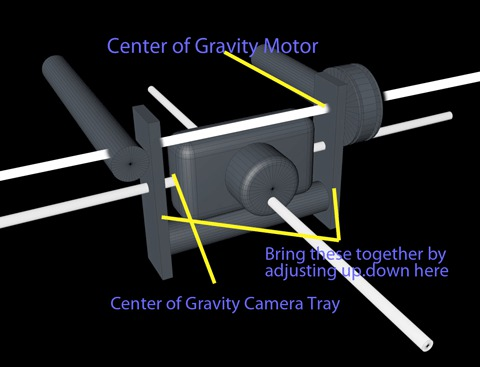
\includegraphics[scale=1.8]{balancing_pitch_1.jpg}
		\end{center}
		\begin{center}
			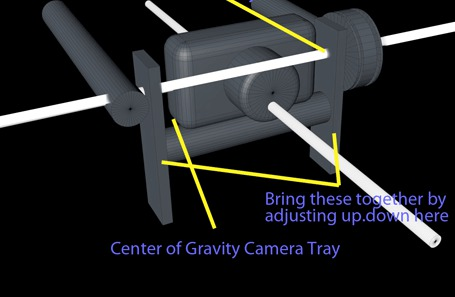
\includegraphics[scale=2.1]{balancing_pitch_2.jpg}
		\end{center}
		\begin{center}
			Balancing pitch axis of the gimbal.
		\end{center}
		\textbf{Balance the Roll axis:}
		\newline
		Follow adjust your gimbal to make sure the COG of the camera is along the motor axis as shown in the image below. Again once its balanced when you change the angle it will stay there when the gimbal is turned off.
		\newline
		\begin{center}
			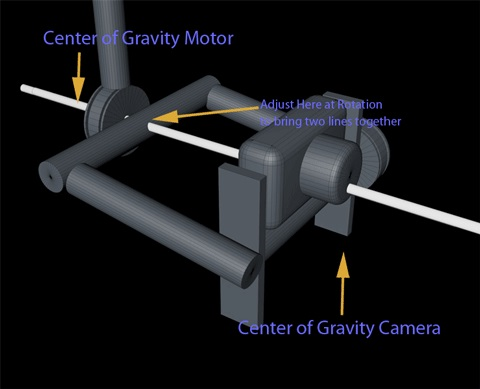
\includegraphics[scale=0.7]{balancing_roll_1.jpg}
		\end{center}
		\begin{center}
			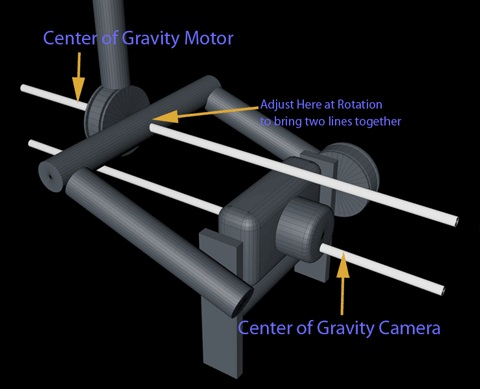
\includegraphics[scale=0.7]{balancing_roll_2.jpg}
		\end{center}
		\begin{center}
			Balancing roll axis of the gimbal.
		\end{center}
		For more details, gifs and videos refer to
		\newline
		\url{http://www.dronetrest.com/t/balancing-your-brushless-gimbal/55}
			
	\section{Experiment}
		\subsection{Making a Gimbal}
		Here I will use some 3D printed parts and some purchased parts for gimbal design. You can make your own 3D design using any 3D design software and then print 3D parts using 3D printing machine or you can use other's 3D designed parts for your gimbal. I got 3D designed parts from \url{http://www.thingiverse.com/thing:1247236} for my 3 axis open brushless gimbal.You can also purchase all the parts. There are many stores are available. Some of them are:
		\begin{itemize}
			\item \url{http://www.hobbyking.com/hobbyking/store/__960__501__Multi_Rotors_Drones_Parts-Camera_Gimbals.html}
			\item \url{http://axisgimbal.com/gimbal-parts} etc.
		\end{itemize}
		%%%%%%%%%%%%%%%%%%%%%%%%%%%%%%%%%%%%%%%%%%%%%%%%%%
		%%%%%%%%%%%%%%%%%%%%%%%%%%%%%%%%%%%%%%%%%%%%%%%%%%
		\textbf{Required 3D printed parts:}
		\newline
		\begin{enumerate}
			%%%%%%%%%%%%%%%%%%%%%%%%%%%%%%%%%%%%%%%%%%%%%%%%%%
			\item \textbf{Vibration and shock observing mounts:} We require two vibration and shock observing mounts.
			\begin{center}
				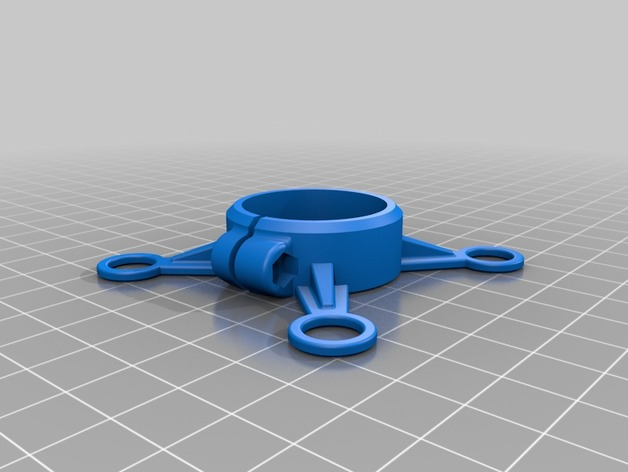
\includegraphics[scale=0.5]{lower_vibration_observing_mount.jpg}
			\end{center}
			\begin{center}
				Lower vibration observing mount.
			\end{center}
			\begin{center}
				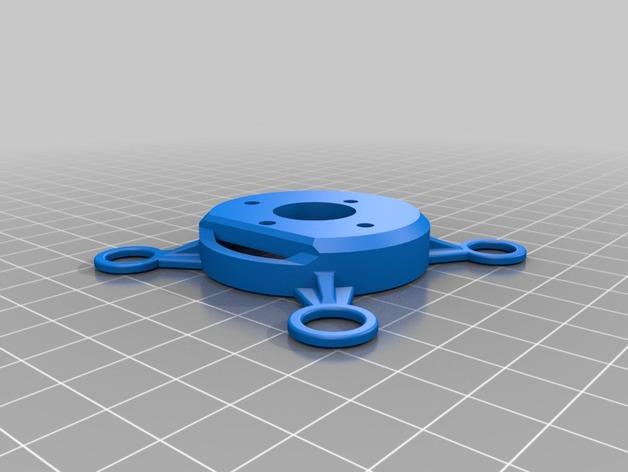
\includegraphics[scale=0.5]{upper_vibration_observing_mount.jpg}
			\end{center}
			\begin{center}
				Upper vibration observing mount.
			\end{center}
			\item \textbf{Gimbal Motor Frame 1:} To hold pitch axis motor.
			\begin{center}
				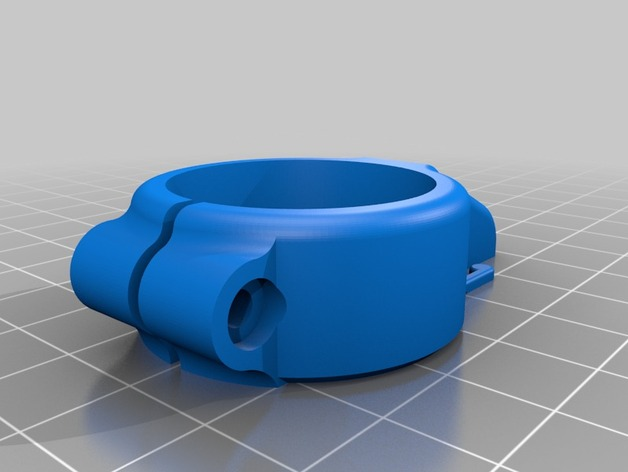
\includegraphics[scale=0.5]{Gimbal_Motor_Frame_1.jpg}
			\end{center}
			\begin{center}
				Gimbal Motor Frame 1.
			\end{center}
			%%%%%%%%%%%%%%%%%%%%%%%%%%%%%%%%%%%%%%%%%%%%%%%%%%
			\item \textbf{Gimbal Motor Frame 2:} To hold roll axis motor.
			\begin{center}
				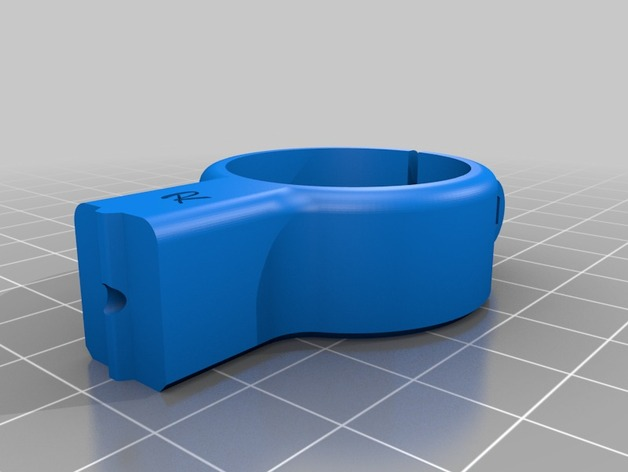
\includegraphics[scale=0.5]{Gimbal_Motor_Frame_2.jpg}
			\end{center}
			\begin{center}
				Gimbal Motor Frame 2.
			\end{center}
			%%%%%%%%%%%%%%%%%%%%%%%%%%%%%%%%%%%%%%%%%%%%%%%%%%
			\item \textbf{Gimbal Motor Frame 3:} To hold yaw axis motor.
			\begin{center}
				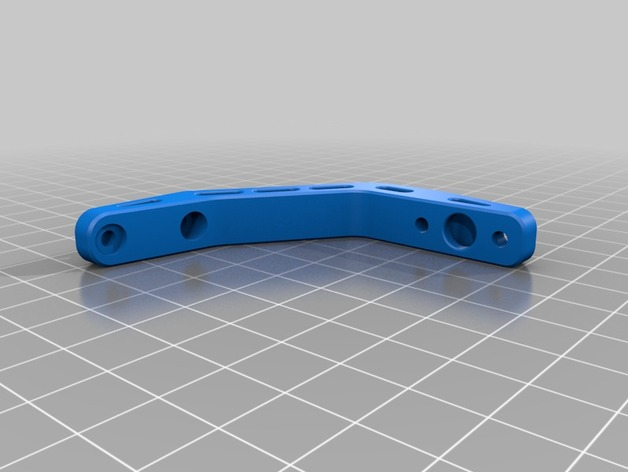
\includegraphics[scale=0.5]{Gimbal_Motor_Frame_3.jpg}
			\end{center}
			\begin{center}
				Gimbal Motor Frame 3.
			\end{center}
			%%%%%%%%%%%%%%%%%%%%%%%%%%%%%%%%%%%%%%%%%%%%%%%%%%
			\item \textbf{Camera Fixing Mount:} To hold camera.
			\begin{center}
				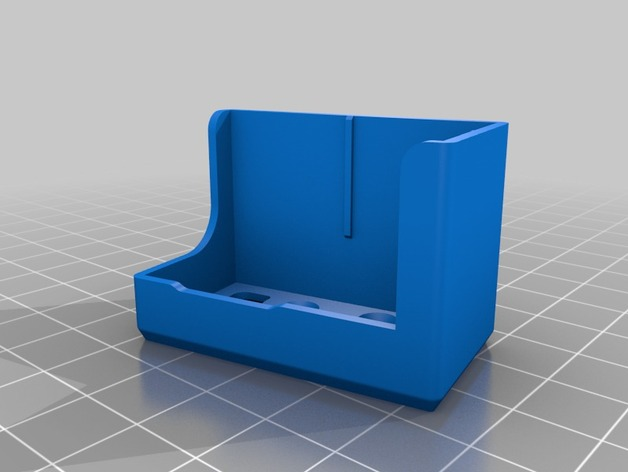
\includegraphics[scale=0.5]{Camera_Fixing_Mount.jpg}
			\end{center}
			\begin{center}
				Camera Fixing Mount.
			\end{center}
		\end{enumerate}
		%%%%%%%%%%%%%%%%%%%%%%%%%%%%%%%%%%%%%%%%%%%%%%%%%%
		%%%%%%%%%%%%%%%%%%%%%%%%%%%%%%%%%%%%%%%%%%%%%%%%%%
		\textbf{Required purchased parts:}
		\newline
		\begin{enumerate}
			%%%%%%%%%%%%%%%%%%%%%%%%%%%%%%%%%%%%%%%%%%%%%%%%%%%
			\item \textbf{Quanum 2208 Precision Brushless Gimbal Motor (GoPRO size 100-200g):} We require 3 Brushless Gimbal Motors to stabilize camera in all Pitch, Roll, and Yaw axises. 
			\par These motors are pre-wound for optimal torque and smoothness. They come with a servo style connector and flexible cable, for plug and play compatibility with most Brushless Gimbal Controllers.
			\par The 2208 is the perfect size for a GoPRO class cameras (100-200g).  It has a superb Fit and Finnish and is engineered to have a lean profile for easy integration into your set-up. The 2208 has preloaded bearings for slop free precision mount, and 14 poles (one of the highest for a motor this size) for ultra-smooth motion. The 2208 brushless gimbal motor is perfect for an upgrade to a kit setup, or the base for a DIY custom gimbal.
			\par It can be found here,
			\newline
			\url{http://www.hobbyking.com/hobbyking/store/__42247__Quanum_2208_Precision_Brushless_Gimbal_Motor_GoPRO_size_100_200g_.html}
			\newline
			\textbf{specs:}
			\begin{itemize}
				\item Camera Range: 100-200 grams (GoPro size)
				\item Poles: 14P12S
				\item KV: 114
				\item Idle current amps: .03A
				\item Resistance: 23mh ohm
				\item Weight: 39 grams
				\item Voltage: 6-14volts (2-3 cell lipoly)
				\item Lower back mounting: 16*19mm
				\item Upper top mounting: 12mm hole to hole
				\item Connection: 3 wire servo style connection 190mm long leads
				\item Mounting Thread: M3
			\end{itemize}
			\begin{center}
				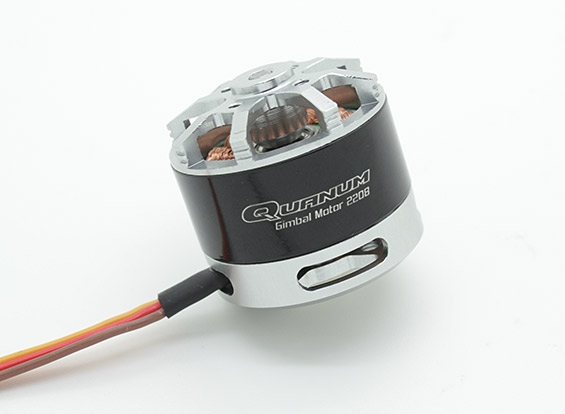
\includegraphics[scale=0.3]{Brushless_Gimbal_Motor.jpg}
			\end{center}
			\begin{center}
				Quanum 2208 Precision Brushless Gimbal Motor (GoPRO size 100-200g).
			\end{center}
			%%%%%%%%%%%%%%%%%%%%%%%%%%%%%%%%%%%%%%%%%%%%%%%%%%%
			\item \textbf{Storm 32 3 Axis Brushless Gimbal Controller:} To control motors.
			\par The Storm 32 3 Axis BGC is a high quality DIY brushless gimbal controller that offers unparalleled professional stabilisation properties at 32Bit level. The Storm 32 board also features an integrated HC06 Blue tooth unit which allows you to program the board wirelessly without any cable connections.
			\par The Storm 32 has a 32Bit microprocessor which operates at 72MHz and provides sufficient power to your DIY gimbal assembly. The 32Bit microprocessor and firmware combined provides an incredible range of programming functions.
			\par The on board output options provide a multitude of connectivity options including PWM, PPM, IR LEDs, joystick, button, 7 x auxiliary ports which can be used as inputs and/or outputs for PWM/Sum-PPM signals. The Storm 32 also supports the connection of a range of satellite receivers including Futaba S-Bus and Spektrum types.
			\textbf{Features:}
			\begin{itemize}
				\item Processor: STM32F103RC at 72Mhz
				\item Motor driver: DRV8313 with short circuit, overheat protection
				\item On board gyro and acceleration sensor MPU6050
				\item IR LED Interface
				\item Futaba S-BUS Compatible / Spektrum satellite port
				\item 7CH PWM/Sum-PPM input/output
			\end{itemize}
			\textbf{Specifications:}
			\begin{itemize}
				\item Power Supply: 12v (3S)
				\item Drive Current: Max 1.5A
				\item Dimensions: 50 x 50mm
				\item Weight: 10g
				\item Mount Holes: M3
			\end{itemize}
			\textbf{Package Includes:}
			\begin{itemize}
				\item 1 x Brushless controller
				\item 1 x Controller case
				\item 1 x MPU6050 sensor
				\item 1 x Sensor case
				\item 1 x Sensor connecting cable
				\item 1 x Pin set
			\end{itemize}
			It can be found here,
			\newline
			\url{http://www.hobbyking.com/hobbyking/store/__84191__Storm_32_3_Axis_Brushless_Gimbal_Controller.html}
			\begin{center}
				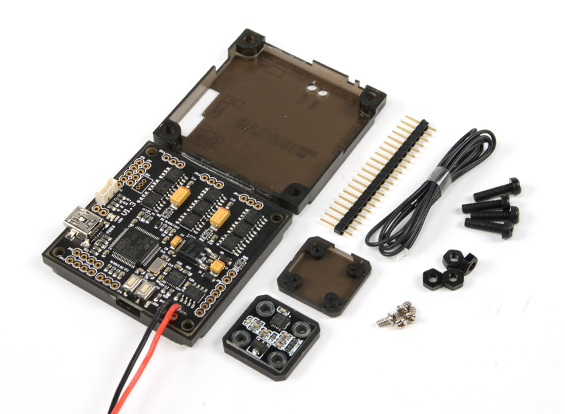
\includegraphics[scale=0.3]{Controller.jpg}
			\end{center}
			\begin{center}
				Storm 32 3 Axis Brushless Gimbal Controller.
			\end{center}
			%%%%%%%%%%%%%%%%%%%%%%%%%%%%%%%%%%%%%%%%%%%%%%%
			\item \textbf{DJI H3-3D Standard Version Part42 Damping Shock Absorber Ball:} We require 4 balls to stay gimbal shock free. It can be found here,
			\newline
			\url{http://www.amazon.com/DJI-Standard-Version-Damping-Absorber/dp/B00RCAOPEI} 
			\begin{center}
				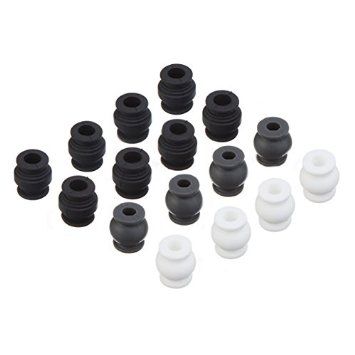
\includegraphics[scale=0.5]{Shock_Absorber_Balls.jpg}
			\end{center}
			\begin{center}
				Figure: DJI H3-3D Standard Version Part42 Damping Shock Absorber Balls.
			\end{center}
			%%%%%%%%%%%%%%%%%%%%%%%%%%%%%%%%%%%%%%%%%%%%%%%
			\item \textbf{Stainless Steal Bolts:} We require,
			\begin{itemize}
				\item 3x M3 x 20mm HEX button head (for the motor clamps)
				\item 1x M3 x 20mm HEX button head (for the frame 1-frame 2 connection)
				\item 4x M3 x 8mm HEX button head (for the gimbal motor frame 3)
				\item 4x M3 x 6mm HEX flat head (for the camera fixing mount)
			\end{itemize}
			%%%%%%%%%%%%%%%%%%%%%%%%%%%%%%%%%%%%%%%%%%%%%%%
		\end{enumerate}
		%%%%%%%%%%%%%%%%%%%%%%%%%%%%%%%%%%%%%%%%%%%%%%%
		%%%%%%%%%%%%%%%%%%%%%%%%%%%%%%%%%%%%%%%%%%%%%%%
		\textbf{Gimbal Making Process:}
		\newline
		Now work is very simple. What you have to do is assembling of parts. First of all mount all three motors on all three gimbal motor frames and assemble them using screws and attach lower vibration observing mount to upper motor using bolts and screws. So your gimbal will be like:
		\begin{center}
			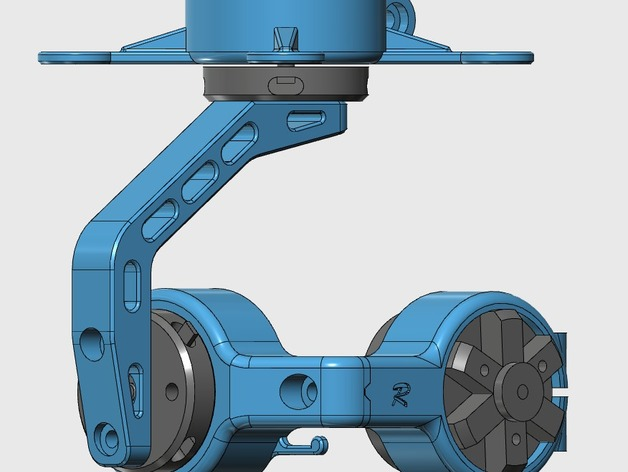
\includegraphics[scale=0.5]{gimbal_making_phase_1.jpg}
		\end{center}
		\begin{center}
			Figure: Phase 1 Gimbal.
		\end{center}
		Now attach damping shock observer balls ans upper vibration observing mount to the gimbal. Then attach camera fixing mount to your gimbal using bolts. Your final gimbal will be like:
		\begin{center}
			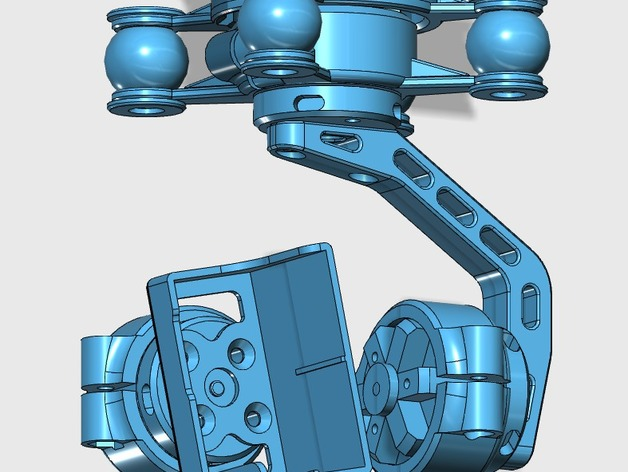
\includegraphics[scale=0.5]{Final_Gimbal.jpg}
		\end{center}
		\begin{center}
			Figure: Final Gimbal.
		\end{center}
		Now you will have to balance your gimbal according to what given in section theory and description.
		%%%%%%%%%%%%%%%%%%%%%%%%%%%%%%%%%%%%%%%%%%%%%%%
		%%%%%%%%%%%%%%%%%%%%%%%%%%%%%%%%%%%%%%%%%%%%%%%
		%%%%%%%%%%%%%%%%%%%%%%%%%%%%%%%%%%%%%%%%%%%%%%%
	\section{Compatible Camera}
		\begin{itemize}
			\item This gimbal is made for GoPro Hero3. So it is best for GoPro Hero3. But you can use any similar size GoPro camera because Camera Fixing Mount is fixed.
			\item You can also use DYS HDV-1 AERIAL VIDEO DRONE and ACTION CAMERA. That is a replacement for GoPro. It can be found at
			\newline
			\url{http://robokits.co.in/quadrotors-hexarotors-drones/fpv-video-telemetry-osd/dys-hdv-1-aerial-video-drone-action-camera-gopro-replacement?gclid=CjwKEAjw4dm6BRCQhtzl6Z6N4i0SJADFPu1nRx_Fo9jfIlLykMuizjcP-umoKJ5WaOs01bwGvmfgNhoC66Hw_wcB\&zenid=do0c7r2d5u3edfg460dpff1qi4}
			\item You can also use any webcam that is compatible for your OS by making or 3D printing a box for camera that can be fixed on camera fixing mount.
		\end{itemize}
	%%%%%%%%%%%%%%%%%%%%%%%%%%%%%%%%%%%%%%%%%%%%%%%
	%%%%%%%%%%%%%%%%%%%%%%%%%%%%%%%%%%%%%%%%%%%%%%%
	%%%%%%%%%%%%%%%%%%%%%%%%%%%%%%%%%%%%%%%%%%%%%%%
	\section{Exercise}
	Some pictures of gimbal balncing the camera are as follows:
	\begin{center}
		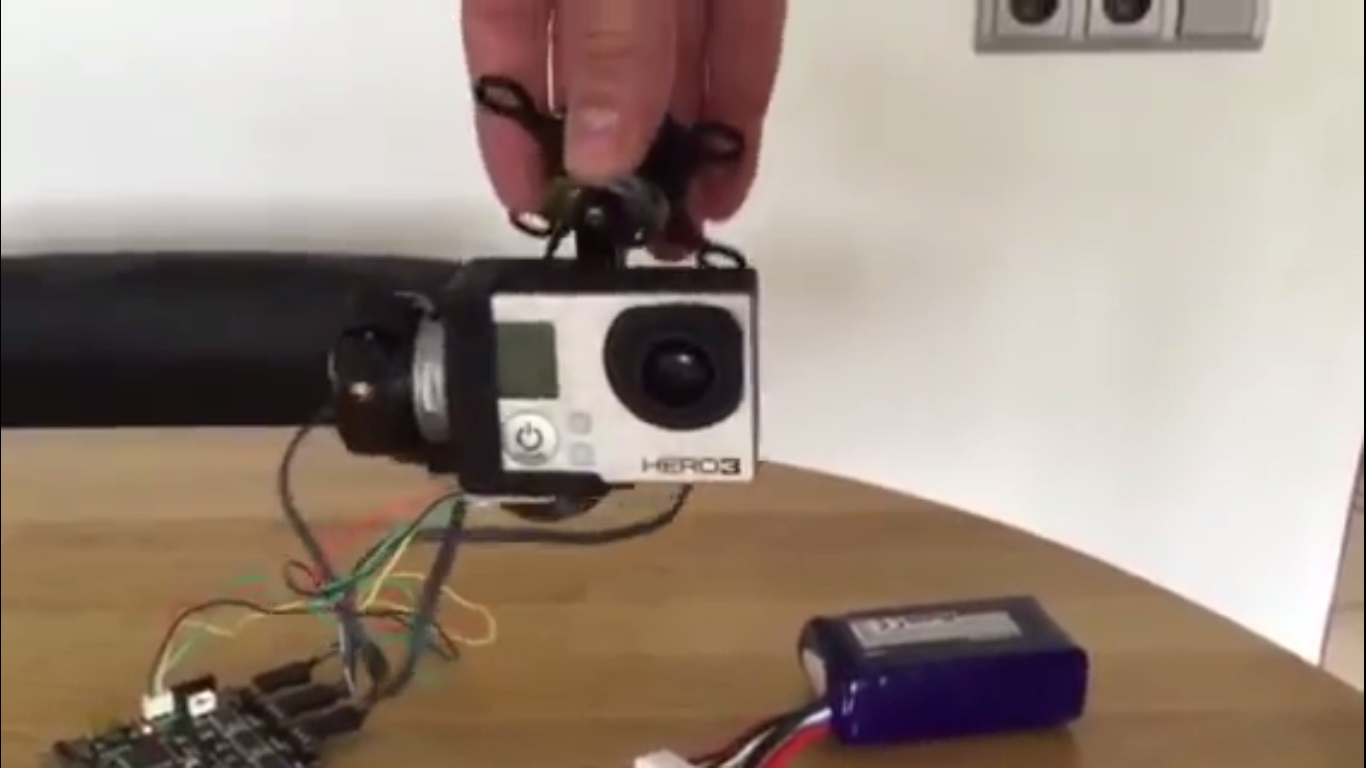
\includegraphics[scale=0.4]{balancing_pitch_axis.jpg}
	\end{center}
	\begin{center}
		Figure: Camera balancing pitch axis.
	\end{center}
	\begin{center}
		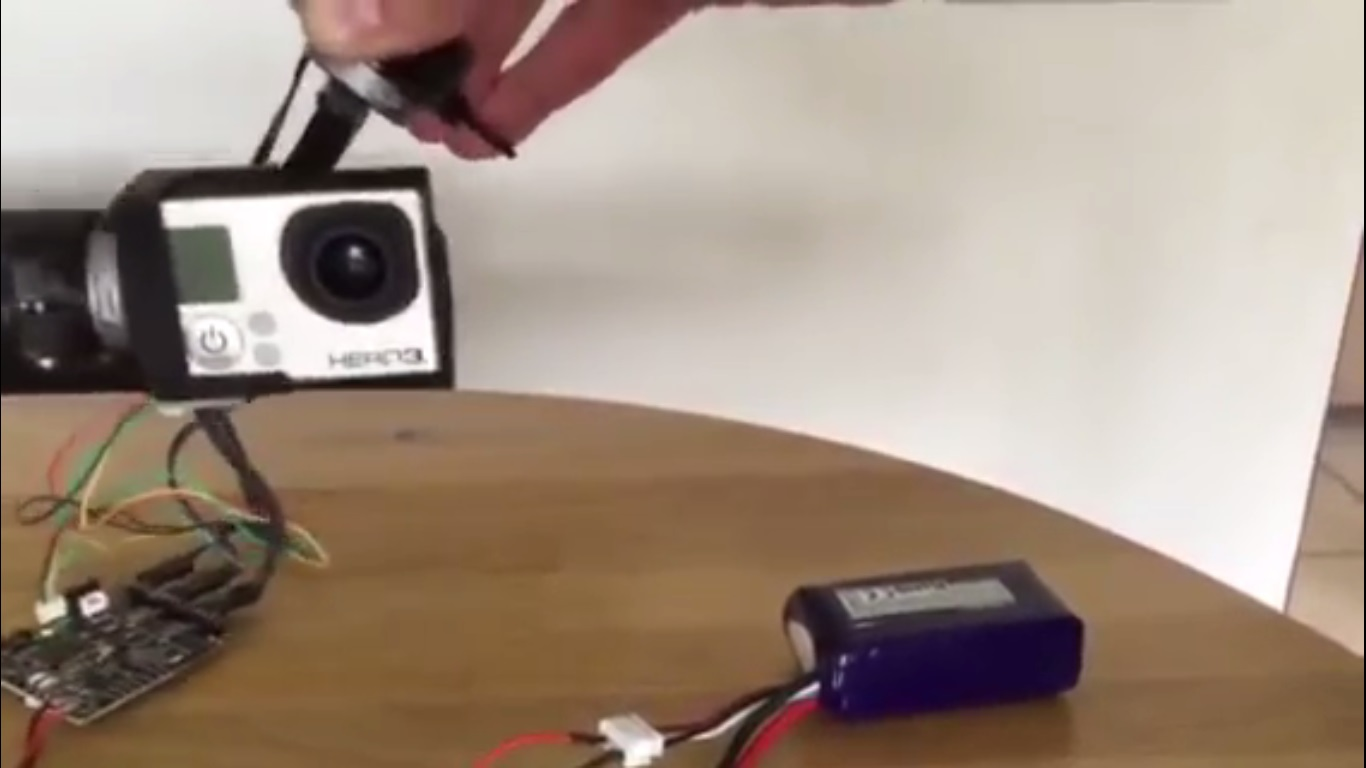
\includegraphics[scale=0.4]{balancing_roll_axis.jpg}
	\end{center}
	\begin{center}
		Figure: Camera balancing roll axis.
	\end{center}
	\begin{center}
		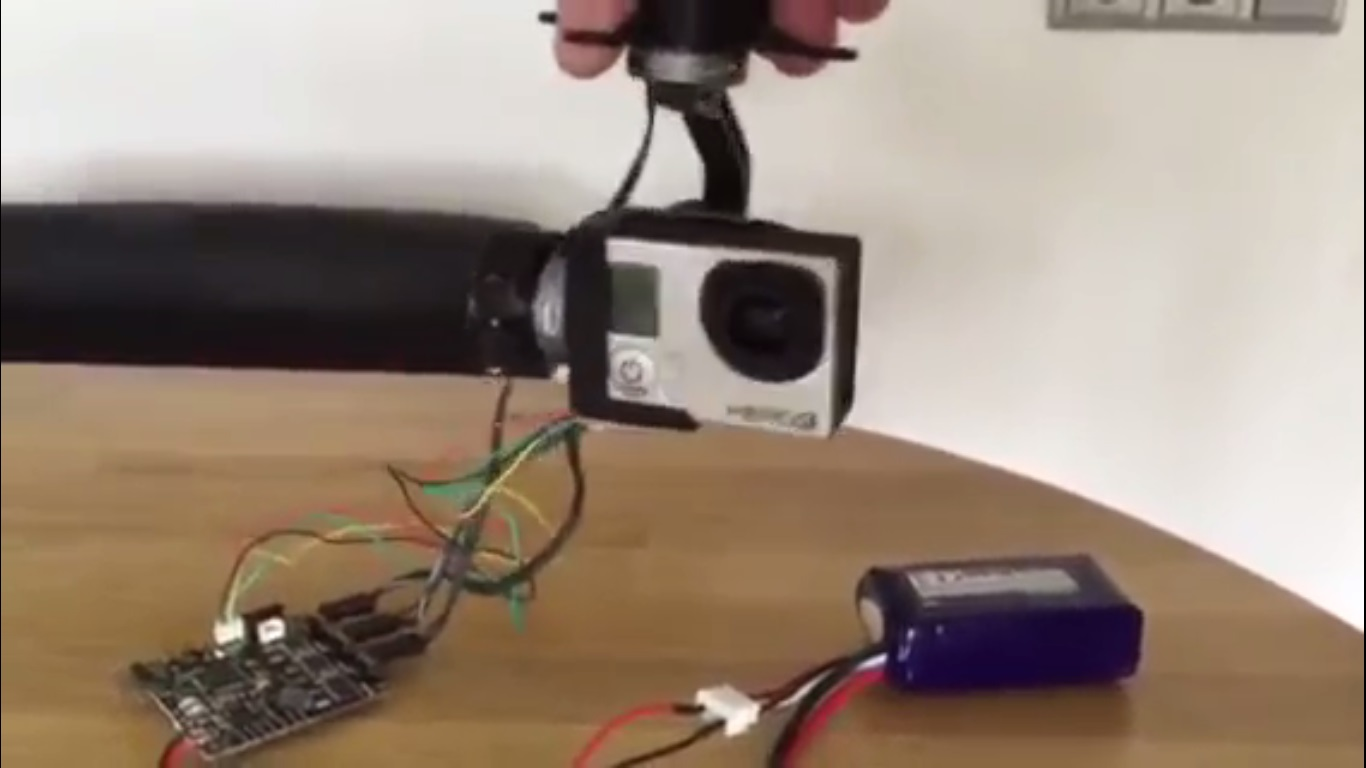
\includegraphics[scale=0.4]{balancing_yaw_axis.jpg}
	\end{center}
	\begin{center}
		Figure: Camera balancing yaw axis.
	\end{center}
	\section{References}
	\begin{itemize}
		\item \url{http://www.hobbyking.com/hobbyking/store/__964__960__Multi_Rotors_Drones_Parts-Gimbal_Accessories.html}
		\item \url{http://www.thingiverse.com/thing:1247236}
		\item \url{http://science.howstuffworks.com/gimbal.htm}
		\item \url{https://en.wikipedia.org/wiki/Gimbal}
		\item \url{http://quadcopterhq.com/what-is-a-gimbal/}
		\item \url{https://en.wikipedia.org/wiki/Rolling_shutter}
		\item \url{http://g03.a.alicdn.com/kf/HTB193EVHFXXXXXTXVXXq6xXFXXXb/FPV-font-b-2-b-font-font-b-Axis-b-font-Brushless-font-b-Gimbal-b.jpg}
		\item \url{http://www.dronetrest.com/t/balancing-your-brushless-gimbal/55}
		\item \url{http://axisgimbal.com/gimbal-parts/}
		\item \url{http://www.hobbyking.com/hobbyking/store/__960__501__Multi_Rotors_Drones_Parts-Camera_Gimbals.html}
		\item \url{http://www.hobbyking.com/hobbyking/store/__42247__Quanum_2208_Precision_Brushless_Gimbal_Motor_GoPRO_size_100_200g_.html}
		\item \url{http://www.hobbyking.com/hobbyking/store/__84191__Storm_32_3_Axis_Brushless_Gimbal_Controller.html}
		\item \url{http://robokits.co.in/quadrotors-hexarotors-drones/fpv-video-telemetry-osd/dys-hdv-1-aerial-video-drone-action-camera-gopro-replacement?gclid=CjwKEAjw4dm6BRCQhtzl6Z6N4i0SJADFPu1nRx_Fo9jfIlLykMuizjcP-umoKJ5WaOs01bwGvmfgNhoC66Hw_wcB&zenid=do0c7r2d5u3edfg460dpff1qi4}
		\item \url{https://www.youtube.com/watch?v=80s-3GhD2zk&feature=youtu.be}
	\end{itemize}
\end{document}